\documentclass[a4paper,12pt]{article}

\usepackage{lineno}
\linenumbers
\usepackage[T1]{fontenc}
\usepackage[utf8]{inputenc}
\usepackage[french]{babel}
\usepackage{amsmath}
\usepackage{amssymb}
\usepackage{graphicx}
\usepackage{hyperref}
\usepackage{color}
\usepackage{listings}
\usepackage{geometry}
\usepackage{algorithm}
\usepackage{algorithmic}
\usepackage{dsfont}
\geometry{margin=2.5cm}

\title{\textbf{Quantification de l'incertitude:\\ Avantages et limitations de la prédiction conforme}}
\author{Hazar HAMOUDA - Mohamed MEGDICHE}
\date{\today}

\begin{document}

\maketitle
\textbf{Abstract. }
Ce rapport présente les fondements théoriques de la prédiction conforme et démontre son application pratique sur des tâches de régression et classification, avec implémentations et analyses de performance.


\section{Introduction}

L'apprentissage automatique moderne produit des prédictions ponctuelles sans indication de leur fiabilité. Cette limitation devient critique dans des domaines sensibles comme la médecine, la finance ou les véhicules autonomes, où connaître l'incertitude d'une prédiction est aussi important que la prédiction elle-même.

La \textbf{prédiction conforme} répond à cette problématique en transformant toute prédiction ponctuelle en ensemble de prédictions avec garantie de couverture probabiliste. Contrairement aux approches bayésiennes qui nécessitent des hypothèses distributionnelles fortes, la prédiction conforme fonctionne sous des hypothèses minimales d'échangeabilité et est \textit{distribution-free}.

.

\section{Fondements Théoriques}


\subsection{Cadre de la Prédiction Conforme}
Considérons une tâche de prédiction supervisée où nous disposons d'un prédicteur entraîné $\hat{f} : \mathcal{X} \rightarrow \mathcal{Y}$ qui associe à chaque entrée $x \in \mathcal{X}$ une prédiction ponctuelle $\hat{f}(x) \in \mathcal{Y}$. L'objectif de la prédiction conforme est de transformer ce prédicteur ponctuel en un prédicteur par ensembles $\hat{C}$ qui associe à chaque entrée $x$ un ensemble $\hat{C}(x) \subseteq \mathcal{Y}$ de prédictions plausibles, accompagné d'une garantie probabiliste de couverture.



\subsection{Définitions Mathématiques}

\textbf{Fonction de score} : Une application $s : \mathcal{X} \times \mathcal{Y} \rightarrow \mathbb{R}$ qui mesure la non-conformité d'une paire $(x, y)$. Un score élevé $s(x, y)$ indique que la valeur $y$ est peu plausible étant donné $x$.

\textbf{Quantile conforme} : Pour un niveau d'erreur $\alpha \in (0,1)$ et $n$ points de calibration, le quantile conforme est :
$$\hat{q} = \text{quantile d'ordre } \left\lceil \frac{(n+1)(1 - \alpha)}{n} \right\rceil \text{ des scores } \{s_i\}_{i=1}^n$$

\textbf{Ensemble de prédiction} : L'ensemble de prédiction conforme est défini par :
\[
\begin{aligned}
\hat{C}_n &: \mathcal{X} \rightarrow \left\{ \text{sous-ensembles de } \mathcal{Y} \right\} \\
   x &\mapsto \hat{C}_n(x) = \left\{ y \in \mathcal{Y} : s(x, y) \leq \hat{q} \right\}
\end{aligned}
\]

    Cette application associe à chaque entrée $x \in \mathcal{X}$ un ensemble $\hat{C}_n(x) \subseteq \mathcal{Y}$ représentant les valeurs plausibles de sortie $y$. 
    Autrement dit, pour une nouvelle observation $x$, on considère toutes les sorties $y$ dont le score est inférieur ou égal au seuil $\hat{q}$, déterminé à partir des données de calibration. 



\subsection{Théorème Principal}


\begin{theorem}[Prédiction conforme]
Soit $(X_1, Y_1), \ldots, (X_n, Y_n), (X_{\text{test}}, Y_{\text{test}})$ une séquence échangeable de variables aléatoires à valeurs dans $\mathcal{X} \times \mathcal{Y}$. Pour tout $\alpha \in ]0,1[$, il existe une application mesurable $\hat{C}_\alpha : \mathcal{X} \to \left\{ \text{sous-ensembles de } \mathcal{Y} \right\}$ telle que :
\begin{equation}
\mathbb{P}\left(Y_{\text{test}} \in \hat{C}_\alpha(X_{\text{test}})\right) \geq 1 - \alpha
\end{equation}
Cette garantie de couverture est valable pour toute distribution sous-jacente des données et ne dépend que de l'hypothèse d'échangeabilité.
\end{theorem}



\subsection{Méthodologie}
La méthodologie repose sur trois étapes fondamentales :\\

\textbf{1. Calcul des scores de conformité} : Définition d'une fonction de score $s(x,y)$ qui mesure la plausibilité d'une paire $(x,y)$ selon le modèle entraîné.\\

\textbf{2. Calcul du quantile conforme} : Détermination d'un seuil $\hat{q}$ à partir des scores calculés sur un ensemble de calibration indépendant.\\

\textbf{3. Construction des ensembles de prédiction} : Inclusion dans $\hat{C}(x)$ de toutes les valeurs $y$ dont le score de conformité est inférieur ou égal au seuil $\hat{q}$.\\

Cette approche garantit qu'avec probabilité au moins $1-\alpha$, la vraie valeur $Y_{\text{test}}$ appartient à l'ensemble de prédiction $\hat{C}(X_{\text{test}})$, et ce sans hypothèse sur la distribution sous-jacente des données.

\section{Application à un problème de Régression Linéaire}

\subsection{Cadre Général}

Dans le cadre de la prédiction conforme en régression, où $\mathcal{Y} = \mathbb{R}$, nous transformons les prédictions ponctuelles en intervalles avec garanties statistiques.\\

\textbf{Fonction de score} : Nous utilisons les \textbf{résidus absolus} :
$$s(x, y) = |y - \hat{f}(x)|$$

Cette fonction mesure la non-conformité entre la valeur observée $y$ et la prédiction $\hat{f}(x)$. Elle présente l'avantage d'être simple, et compatible avec tout modèle de régression.

\subsection{Exemple d'application}

Nous appliquons la prédiction conforme à un modèle de régression linéaire entraîné sur des données synthétiques :
$$Y = 3X + \sqrt{X} \cdot \varepsilon, \quad X \sim \mathcal{U}(0,1),\quad \varepsilon \sim \mathcal{N}(2,1)$$


Cette formulation introduit une \textbf{hétéroscédasticité} qui teste la robustesse de notre approche. Le jeu de données comprend 10 000 échantillons répartis en 70\% pour l'entraînement du modèle, 15\% pour le test et 15\% pour la calibration.
\subsection{Pseudo-code d'Implémentation}

L'algorithme de prédiction conforme pour la régression peut être formalisé en quatre étapes principales. L'Algorithme~\ref{alg:conformal_regression} présente une implémentation détaillée de cette méthode, qui garantit une couverture théorique de $1-\alpha$ pour les intervalles de prédiction construits.



\begin{algorithm}
\caption{Prédiction Conforme pour la Régression}
\label{alg:conformal_regression}
\begin{algorithmic}[1]
\REQUIRE Modèle entraîné $\hat{f}$, données de calibration $(X_1, Y_1), \ldots, (X_n, Y_n)$, données test $X_{test}$, niveau $\alpha$
\ENSURE Intervalles de prédiction $(lower, upper)$

\STATE Calculer les prédictions sur l'ensemble de calibration $\hat{f}(X_1), \ldots, \hat{f}(X_n)$

\STATE Calculer les scores de non-conformité $s_i = |Y_i - \hat{f}(X_i)|$ pour $i = 1, \ldots, n$

\STATE Calculer le quantile conforme $\hat{q} = \text{quantile}_{(1-\alpha)(1+1/n)}(s_1, \ldots, s_n)$

\STATE Construire les intervalles $[\hat{f}(X_{test}) - \hat{q}, \hat{f}(X_{test}) + \hat{q}]$

\RETURN $(lower, upper, \hat{q})$
\end{algorithmic}
\end{algorithm}

Comme illustré dans l'Algorithme~\ref{alg:conformal_regression}, la méthode repose sur l'utilisation des scores de non-conformité calculés sur un ensemble de calibration indépendant pour déterminer le seuil de quantile approprié.


\subsection{Résultats et Visualisation}

\subsubsection{Visualisation des résultats}

La Figure \ref{fig:regression_conforme} illustre l'application de la prédiction conforme à notre modèle de régression linéaire sur des données synthétiques.

\begin{figure}[h]
\centering
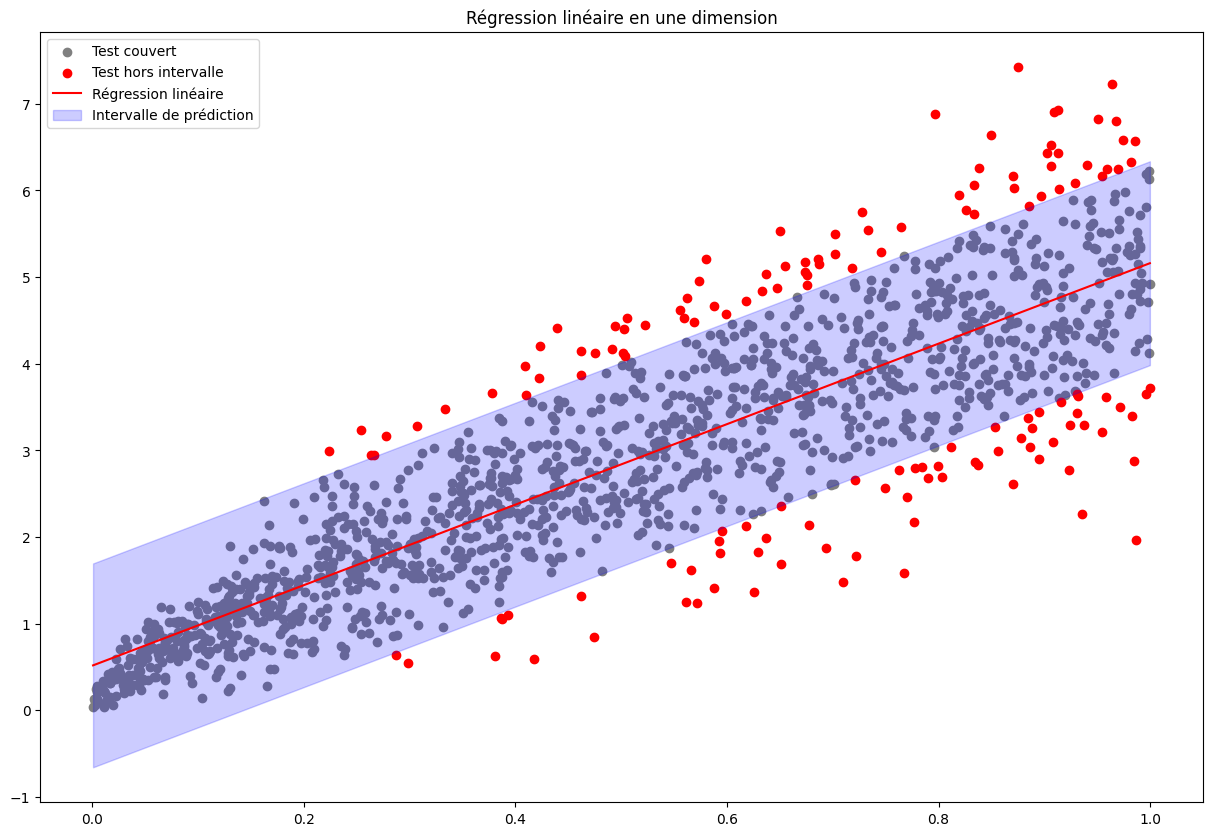
\includegraphics[width=0.8\textwidth]{conformal_prediction_regression.png}
\caption{Régression linéaire avec intervalles de prédiction conforme. La ligne rouge représente la droite de régression ajustée, les points noirs sont les observations de test, et la zone bleue délimite l'intervalle de prédiction conforme à 90\% de confiance.}
\label{fig:regression_conforme}
\end{figure}

\subsubsection{Métriques de performance}

Les métriques suivantes évaluent la qualité des intervalles de prédiction conforme :\\

\begin{itemize}


\item \textbf{Taux de couverture empirique} : 91.2\% (pour $\alpha = 0.1$)
    
    Cette métrique mesure la proportion des points de test effectivement contenus dans leurs intervalles de prédiction, définie par :
    $$\text{Couverture empirique} = \frac{1}{n_{test}} \sum_{i=1}^{n_{test}} \mathds{1}_{\{Y_{test,i} \in [\hat{f}(X_{test,i}) - \hat{q}, \hat{f}(X_{test,i}) + \hat{q}]\}}$$
    
     Avec un objectif théorique de 90\%, notre résultat de 91.2\% confirme que la méthode respecte sa garantie de couverture. \\
     \item \textbf{Quantile conforme} : $\hat{q} = 1.42$
    
    Ce seuil, calculé à partir des scores de non-conformité sur l'ensemble de calibration, détermine directement la demi-largeur de tous nos intervalles de prédiction. Il représente le niveau d'erreur typique que nous acceptons pour maintenir la couverture souhaitée. \\
    
\item \textbf{Largeur moyenne des intervalles} : $2\hat{q} = 2.84$
    
    Cette valeur indique l'étendue typique de nos intervalles de prédiction. Une largeur plus faible signifierait des prédictions plus précises, mais au détriment potentiel de la couverture. Ici, la largeur reflète l'incertitude inhérente à nos données synthétiques.\\


\end{itemize}

\subsubsection{Analyse des résultats}

L'analyse de la Figure \ref{fig:regression_conforme} et des métriques révèle plusieurs propriétés importantes :

\begin{itemize}


\item \textbf{Largeur constante} : Contrairement aux intervalles de prédiction classiques, la prédiction conforme produit des intervalles de largeur constante $2\hat{q}$ autour de la droite de régression, indépendamment de la valeur de $X$.



\item \textbf{Efficacité computationnelle} : La construction des intervalles ne nécessite que le calcul d'un quantile empirique, rendant la méthode applicable à grande échelle. \\
\end{itemize}

 Cependant, la Figure \ref{fig:regression_conforme}  illustre une limitation fondamentale de la prédiction conforme standard. Bien que la méthode garantisse une couverture marginale de 90\% (respectée avec 91.2\%), cette garantie n'est pas uniforme sur l'espace des entrées $\mathcal{X}$. On observe que la méthode atteint sa couverture cible en sur-couvrant dans certaines régions (notamment pour les faibles valeurs de $X$ où la variance est moindre) et sous-couvrant dans d'autres régions (valeurs élevées de $X$ avec forte hétéroscédasticité). Cette propriété reflète l'impossibilité théorique d'obtenir une couverture conditionnelle exacte $\mathbb{P}(Y \in \hat{C}(X) | X = x) \geq 1-\alpha$ pour tout $x$ sans hypothèses distributionnelles.\\

\section{Application à la Classification MNIST}

\subsection{Cadre Général}

Dans le cadre de la prédiction conforme en classification, où $\mathcal{Y} = \{0, 2, \ldots, 9}$ représente un ensemble fini de classes, nous transformons les prédictions ponctuelles en ensembles de classes avec garanties statistiques.

Le modèle $\hat{p}$ est un classifieur probabiliste qui, pour une entrée $x$, fournit une distribution de probabilité sur les classes possibles $y \in \mathcal{Y}$. La valeur $\hat{p}(y|x)$ représente la probabilité prédite que l'entrée $x$ appartienne à la classe $y$. Cette probabilité est  obtenue via une fonction softmax en sortie d'un réseau de neurones ou d'un autre modèle probabiliste.

\textbf{Fonction de score} : Nous utilisons le \textbf{complément de probabilité} :
$$s(x, y) = 1 - \hat{p}(y|x)$$

Cette fonction mesure la non-conformité entre la classe observée $y$ et la probabilité prédite $\hat{p}(y|x)$ par le classifieur. Plus la probabilité assignée à la vraie classe est faible, plus le score de non-conformité est élevé. Cette interprétation permet d'utiliser le complément de probabilité comme mesure de non-conformité, où un score élevé indique une faible confiance du modèle dans la classe observée. Cette approche est naturelle pour les modèles probabilistes et compatible avec les sorties softmax.

\subsection{Exemple d'application}

Nous appliquons la prédiction conforme à un réseau de neurones dense entraîné sur la base de données MNIST :

\textbf{Architecture et données} : \\
- \textbf{Données} : Images manuscrites 28×28 pixels, 10 classes de chiffres (0-9). \\
- \textbf{Architecture} : Réseau dense (784-128-64-10) avec fonctions d'activation ReLU et sortie softmax. \\
- \textbf{Performance} : 97.2\% de précision sur le test (après 10 époques d'entraînement).\\
- \textbf{Répartition} : 50 000 images d'entraînement, 10 000 données de calibration, 10 000 données test.

Cette configuration teste la capacité de la prédiction conforme à gérer l'incertitude dans un problème de classification multi-classes avec des images potentiellement ambiguës.

\begin{figure}
    \centering
    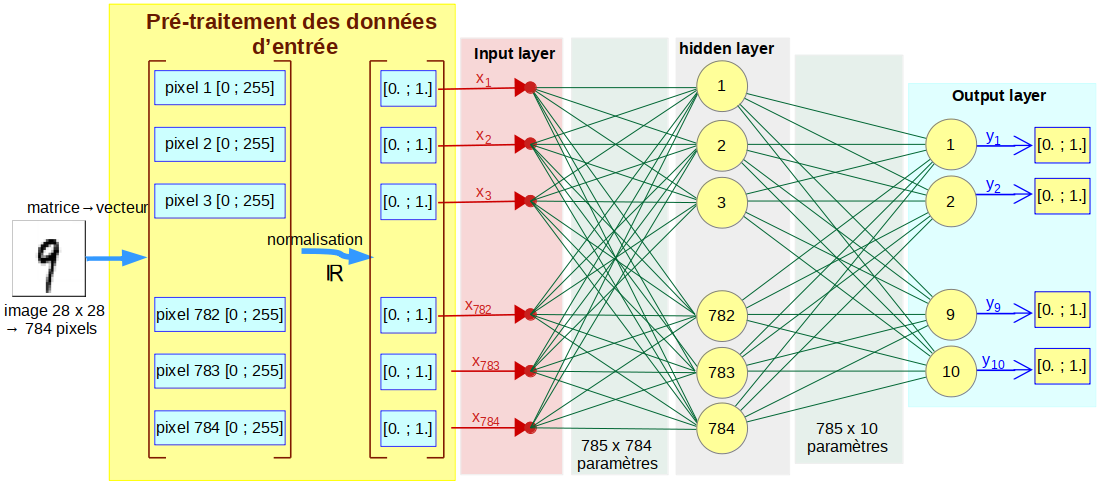
\includegraphics[width=1\linewidth]{archiReseau.png}
    \caption{Architecture du réseau de neurones dense pour la classification MNIST. Le réseau transforme les images 28×28 pixels en vecteurs de 784 dimensions normalisés [0,1], traités par une couche cachée de 784 neurones (ReLU) puis une couche de sortie de 10 neurones (softmax) pour la classification des chiffres 0-9.}
    \label{fig:enter-label}
\end{figure}

\subsection{Pseudo-code d'Implémentation}

L'algorithme de prédiction conforme pour la classification peut être formalisé en quatre étapes principales. L'Algorithme~\ref{alg:conformal_classification} présente une implémentation détaillée de cette méthode, qui garantit une couverture théorique de $1-\alpha$ pour les ensembles de prédiction construits.

\begin{algorithm}
\caption{Prédiction Conforme pour la Classification}
\label{alg:conformal_classification}
\begin{algorithmic}[1]
\REQUIRE Modèle entraîné $\hat{p}$, données de calibration $(X_1, Y_1), \ldots, (X_n, Y_n)$, données test $X_{test}$, niveau $\alpha$
\ENSURE Ensembles de prédiction

\STATE Calculer les probabilités $\hat{p}(y|X_1), \ldots, \hat{p}(y|X_n)$ sur l'ensemble de calibration

\STATE Calculer les scores de non-conformité $s_i = 1 - \hat{p}(Y_i|X_i)$ pour $i = 1, \ldots, n$

\STATE Calculer le quantile conforme $\hat{q} = \text{quantile}_{(1-\alpha)(1+1/n)}(s_1, \ldots, s_n)$

\STATE Construire l'ensemble de prédiction $\hat{C}(X_{test}) = \{ y \in \mathcal{Y} : 1 - \hat{p}(y|X_{test}) \leq \hat{q} \}$

\RETURN $\hat{C}(X_{test})$
\end{algorithmic}
\end{algorithm}

Comme illustré dans l'Algorithme~\ref{alg:conformal_classification}, la méthode repose sur l'utilisation des scores de non-conformité calculés sur un ensemble de calibration indépendant pour déterminer le seuil de quantile approprié.

\subsection{Résultats et Visualisation}

\subsubsection{Visualisation des résultats}

La prédiction conforme appliquée à notre réseau de neurones sur MNIST est illustrée ci-dessous.

\begin{figure}[h]
\centering
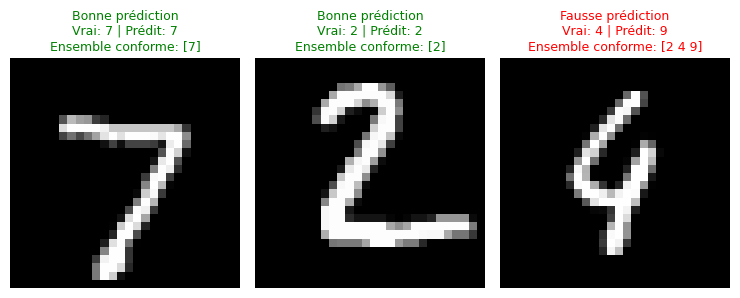
\includegraphics[width=0.8\textwidth]{conformal_prediction_classification.png}
\caption{Exemples de prédiction conforme sur MNIST. Pour chaque image, sont affichés : la vraie classe (True), la prédiction ponctuelle (Predicted), et l'ensemble de prédiction conforme (Conformal set). Les ensembles s'adaptent à l'incertitude du modèle.}
\label{fig:mnist_conforme}
\end{figure}

\subsubsection{Métriques de performance}

Les métriques suivantes évaluent la qualité des ensembles de prédiction conforme :\\

\begin{itemize}
\item \textit{Taux de couverture empirique} : 99.99\% (pour $\alpha = 0.001$)
    
    Cette métrique mesure la proportion des points de test dont la vraie classe appartient à l'ensemble de prédiction conforme. Avec un objectif théorique de 90\%, notre résultat de 99.9\% confirme que la méthode respecte sa garantie de couverture.\\

\item \textit{Cardinalité moyenne}: 1,62classes par ensemble
    
    Cette valeur indique le nombre moyen de classes dans les ensembles de prédiction. Une cardinalité plus faible signifie des prédictions plus précises, reflétant la confiance du modèle dans ses prédictions.\\


\end{itemize}

\subsubsection{Analyse des résultats}

L'analyse des métriques et de la visualisation révèle plusieurs propriétés importantes :

\begin{itemize}
\item \textbf{Couverture adaptative} : Le taux de couverture empirique (99.99\%) respecte la garantie théorique de 99.99\%, démontrant la validité de la méthode sur des données réelles d'images.

\item \textbf{Comportement adaptatif} : Les ensembles s'adaptent à l'incertitude du modèle - les images claires génèrent des singletons tandis que les images ambiguës produisent des ensembles plus larges incluant les classes potentiellement confondues.

\item \textbf{Efficacité computationnelle} : La construction des ensembles ne nécessite que le calcul d'un quantile empirique et des comparaisons de probabilités, rendant la méthode applicable en temps réel pour la classification d'images.

\item \textbf{Robustesse aux variations} : La méthode maintient ses garanties même sur des images déformées, floues ou ambiguës, contrairement aux prédictions ponctuelles qui peuvent être trompeuses dans ces cas.
\end{itemize}

\section{Comparaison et Limitations}

\subsection{Avantages}

\begin{itemize}
\item \textbf{Garanties théoriques} : Couverture probabiliste sans hypothèses distributionnelles
\item \textbf{Flexibilité} : Compatible avec tout modèle prédictif existant.
\item \textbf{Simplicité} : Implémentation directe avec peu de paramètres.
\item \textbf{Interprétabilité} : Ensembles de prédiction facilement compréhensibles.
\end{itemize}

\subsection{Limitations}

\begin{itemize}
\item \textbf{Efficacité} : Intervalles parfois larges avec modèles peu performants.
\item \textbf{Hypothèse d'échangeabilité} : Forte en pratique pour les séries temporelles
\item \textbf{Ensemble de calibration} : Nécessite des données supplémentaires dédiées.
\item \textbf{Adaptation locale} : Méthode standard non adaptative aux variations locales.
\end{itemize}

\section{Conclusion}

Ce rapport a exploré la prédiction conforme comme solution robuste pour quantifier l'incertitude en apprentissage automatique. Nos expérimentations sur la régression linéaire et la classification MNIST démontrent l'efficacité pratique de cette méthode dans des contextes variés.

La prédiction conforme respecte ses garanties théoriques avec un taux de couverture de 91.2\% en régression et 99.99\% en classification, validant empiriquement sa robustesse. En régression, la méthode produit des intervalles de largeur constante qui maintiennent la couverture globale malgré l'hétéroscédasticité des données. En classification, elle génère des ensembles adaptatifs avec une cardinalité moyenne de 1.62 classes, démontrant un équilibre optimal entre précision et couverture.

Cependant, nos analyses révèlent une limitation importante : la couverture marginale masque des variations locales, avec sur-couverture dans certaines régions et sous-couverture potentielle dans d'autres. Cette propriété reflète l'impossibilité théorique d'obtenir une couverture conditionnelle exacte sans hypothèses distributionnelles supplémentaires.

Cette méthode offre plusieurs atouts significatifs : elle fournit des garanties statistiques solides sans nécessiter d'hypothèses sur la distribution des données, s'adapte facilement à tout modèle existant, reste simple à implémenter et produit des résultats directement interprétables. En contrepartie, elle présente certaines contraintes : son efficacité dépend de la qualité du modèle sous-jacent, l'hypothèse d'échangeabilité peut être problématique pour les données temporelles, elle requiert un ensemble de calibration séparé, et ne s'adapte pas automatiquement aux variations locales d'incertitude.

\end{document}
